\section{Speed Optimization Experiments}

\subsection{Memory}
The main blocks of memory in the C++ code is fixed in compile-time and is and
parametrized by the size of the system, 14x14 in the case of the Chicago
trifocal problem:
\begin{verbatim}
complex Hxt[(14+1)*14];         // 210
complex x0t0xtblock[2*(14+1)];  // 30
complex dxdt[15];           
complex dxi[14];
\end{verbatim}
The block Hxt, for instance, stores both $H_x$ and $H_t$. The remaining
variables should be self-explanatory.
We first analyze the memory layout of the arrays used for calculation. Each
array element is of complex type double precision, occupying 16 bytes on a
64-bit GNU/Linux system.
\tiny\begin{verbatim}
    sizeof(C<double>) == 16 bytes and sizeof(double) ==  8 bytes

    x0t0xtblock[2*NVEPLUS1]: 30 elements
    0         1         ...       14        15        ...
    +---------+---------+---------+---------+---------+---------+
    |C<double>|C<double>|   ...   |C<double>|C<double>|   ...   |
    |         |         |   ...   | R  |  I |         |   ...   |
    +---------+---------+---------+---------+---------+---------+
    ^                              ^               ^
    | x0t                          | t0            | xt
    | x0                             (double *)    | x1t1

    Hxt[NVEPLUS1*f::nve]: 15 * 14 == 210 elements
    0         1         ...       14        15        ...       196       ...
    +---------+---------+---------+---------+---------+---------+---------+---------+
    |C<double>|C<double>|   ...   |C<double>|C<double>|   ...   |C<double>|   ...   |
    |         |         |   ...   |         |         |   ...   |         |   ...   |
    +---------+---------+---------+---------+---------+---------+---------+---------+
    ^                                                           ^
    | HxH                                                       | RHS
    dxdt[NVEPLUS1]: 15 elements
    0         1         ...       14        15
    +---------+---------+---------+---------+---------+
    |C<double>|C<double>|   ...   |C<double>|C<double>|
    |         |         |   ...   | R  |  I |         |
    +---------+---------+---------+---------+---------+
    ^                              ^
    | dx                           | dt
    | dx4                            (double *)

    dxi[f::nve]: 14 elements
    0         1         ...        14
    +---------+---------+---------+---------+
    |C<double>|C<double>|   ...   |C<double>|
    +---------+---------+---------+---------+
\end{verbatim}
\normalsize

By using a ``release with debug info'' build compiled under
\verb|GCC 7.5.0 x86_64-linux-gnu|, we can check the starting addresses of
each array with a debugger. By doing so, we find that there's a gap between,
\verb|x0t0xtblock| and \verb|Hxt| of 3264 bytes (204 elements).
We detected a memory layout gap and tried to eliminate it by implementing a
single, monolithic memory block and managing it ourselves:
\footnotesize\begin{verbatim}

    MEMORY LAYOUT
    (range is inclusive: low <= x <= high):

    0x7fff f7a5 0000
          |
    +-----------+
    | 6100-61df | dxi
    +-----------+
    | 61e0-62cf | dxdt
    +-----------+
    | 62d0-64af | x0t0xtblock
    +-----------+
          |
      64b0-716f   GAP
          |
    +-----------+
    | 7170-7f2f | Hxt
    +-----------+
\end{verbatim}
\normalsize
The speedup in defining a single contiguous block was promising but dependent on the compiler.

\subsection{Valgrind}

Valgrind is a instrumentation framework and library of dynamic analysis tools.
By using Valgrind's capabilities, we can get further insight into the behavior
of the program during runtime. We used Memcheck to first check for any possible
memory leaks, but none were found.
\begin{figure}[H]
  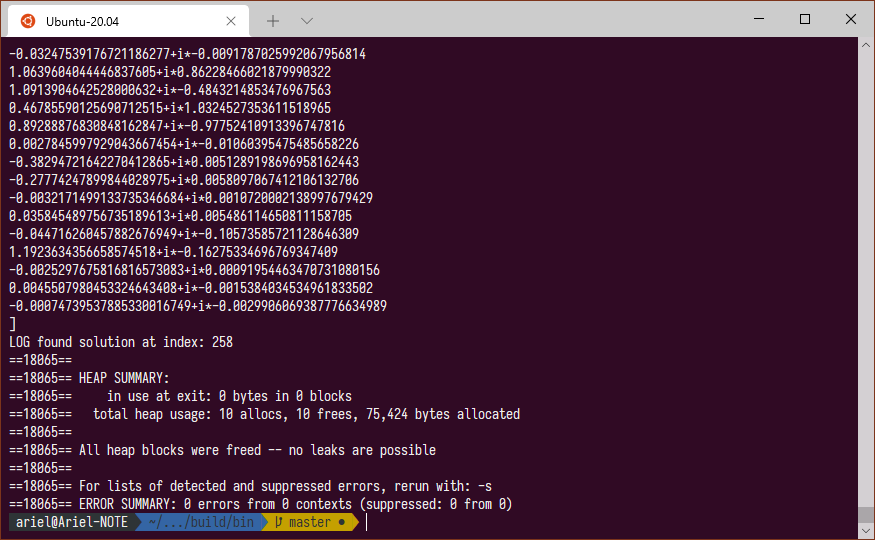
\includegraphics[width=0.8\columnwidth]{figs/valgrind_memcheck}
    \caption{Valgrind Memcheck results}
\end{figure}
Next, we used Cachegrind to check for cache access, cache misses and branch
mispredictions, of which both were under 4\%.
\begin{figure}[H]
  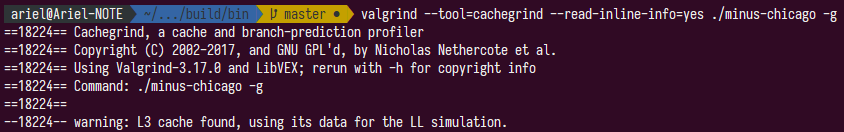
\includegraphics[width=0.8\columnwidth]{figs/valgrind_cachegrind}
  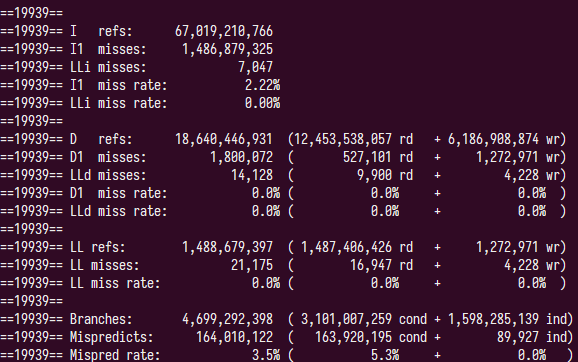
\includegraphics[width=0.8\columnwidth]{figs/valgrind_cachegrind_results}
\caption{Valgrind Cachegrind results}
\end{figure}
The tool Gg\_annotate allows for deeper understanding of the cache access
patterns which can be used to optimize memory access within functions.
\begin{figure}[H]
  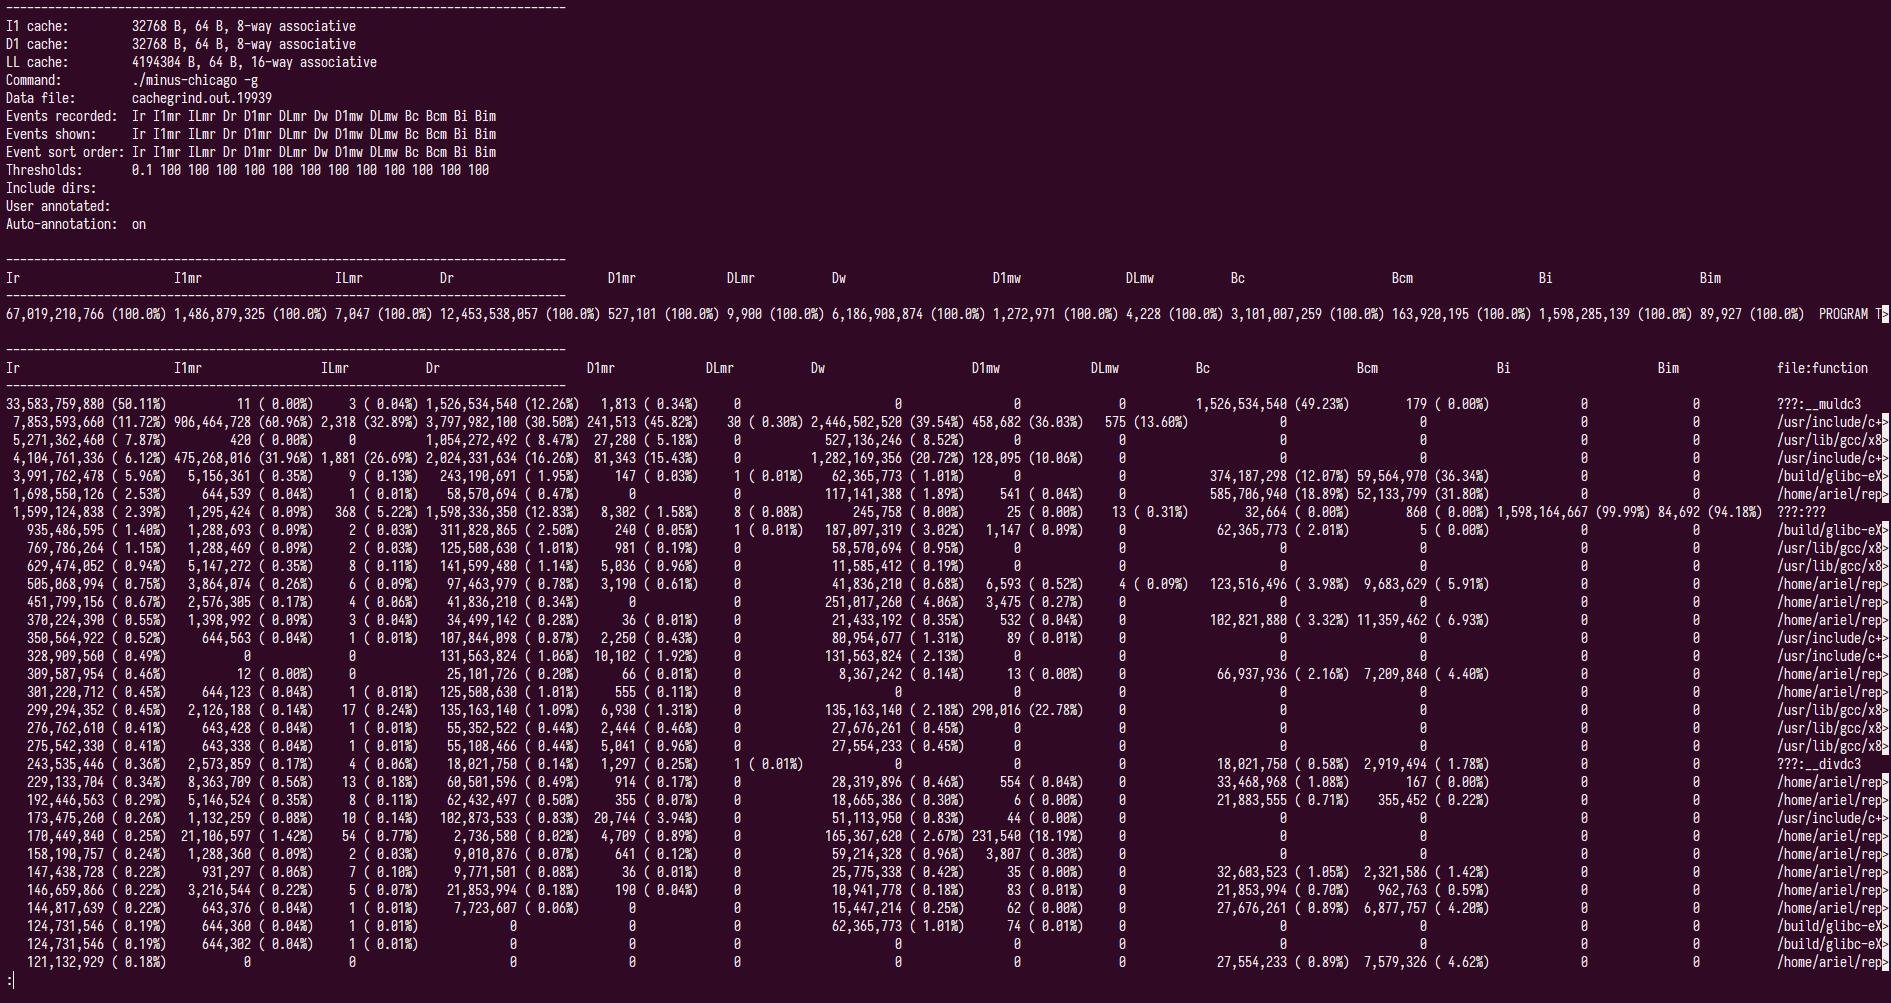
\includegraphics[width=\columnwidth]{figs/valgrind_cg_annotate0}
  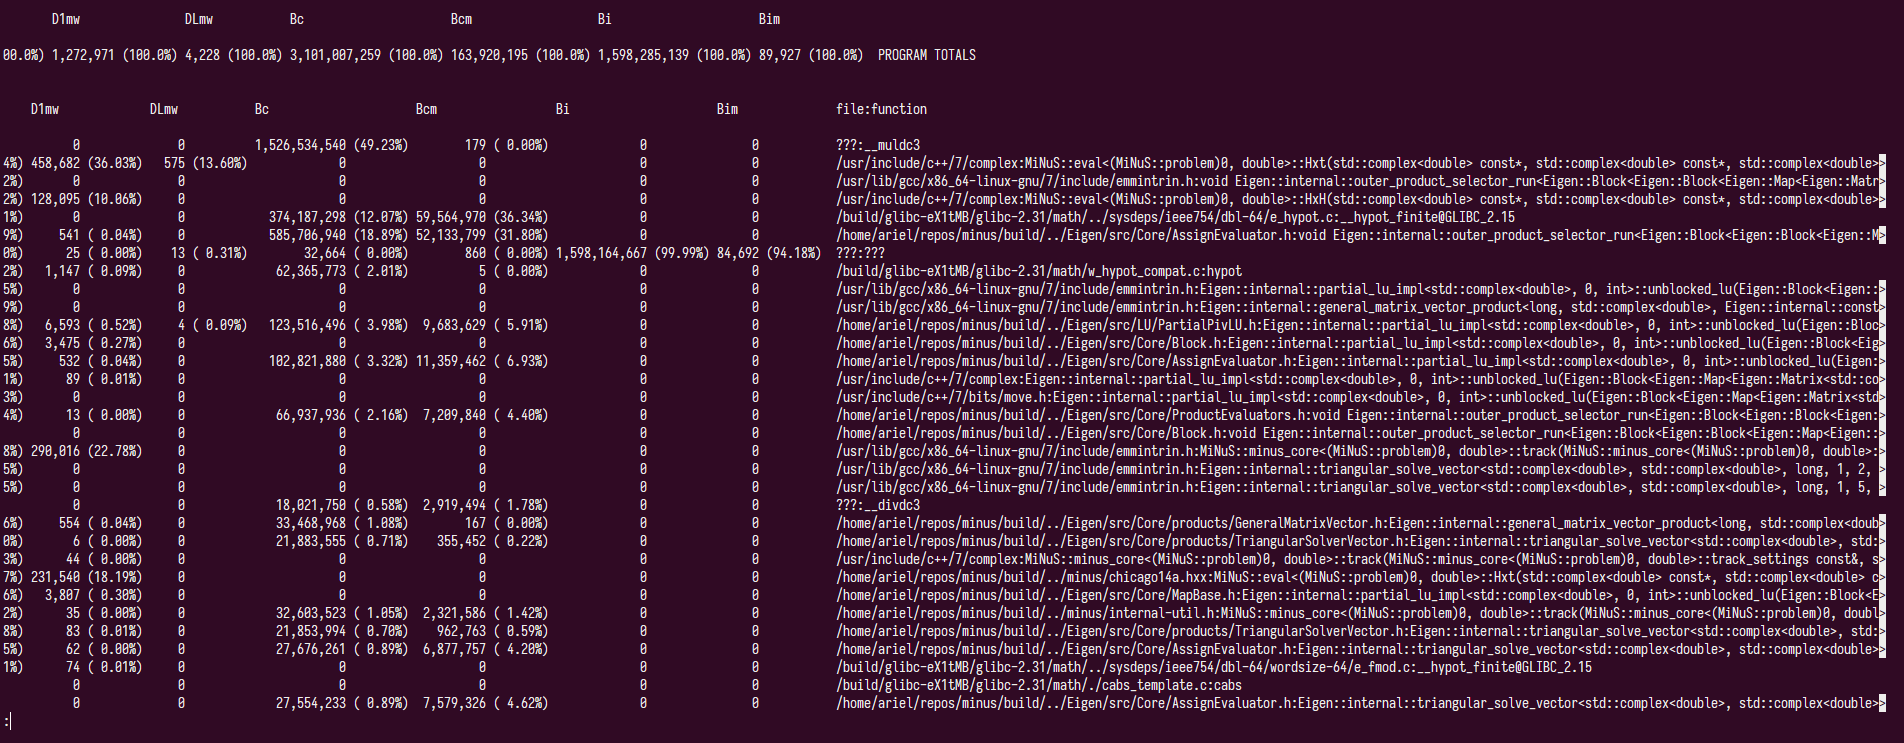
\includegraphics[width=\columnwidth]{figs/valgrind_cg_annotate1}
    \caption{Valgrind Cg\_annotate (Cachegrind\_annotate)}
\end{figure}
Using Callgrind in conjunction with the graphical tool QCachegrind, we can
see the function callers and callees, and what percentage of the total runtime
each one took. From this analysis, we can find that the most used function is
the GCC's library built-in complex multiplication routine, followed by the Eigen
library internal functions.
\begin{figure}[H]
    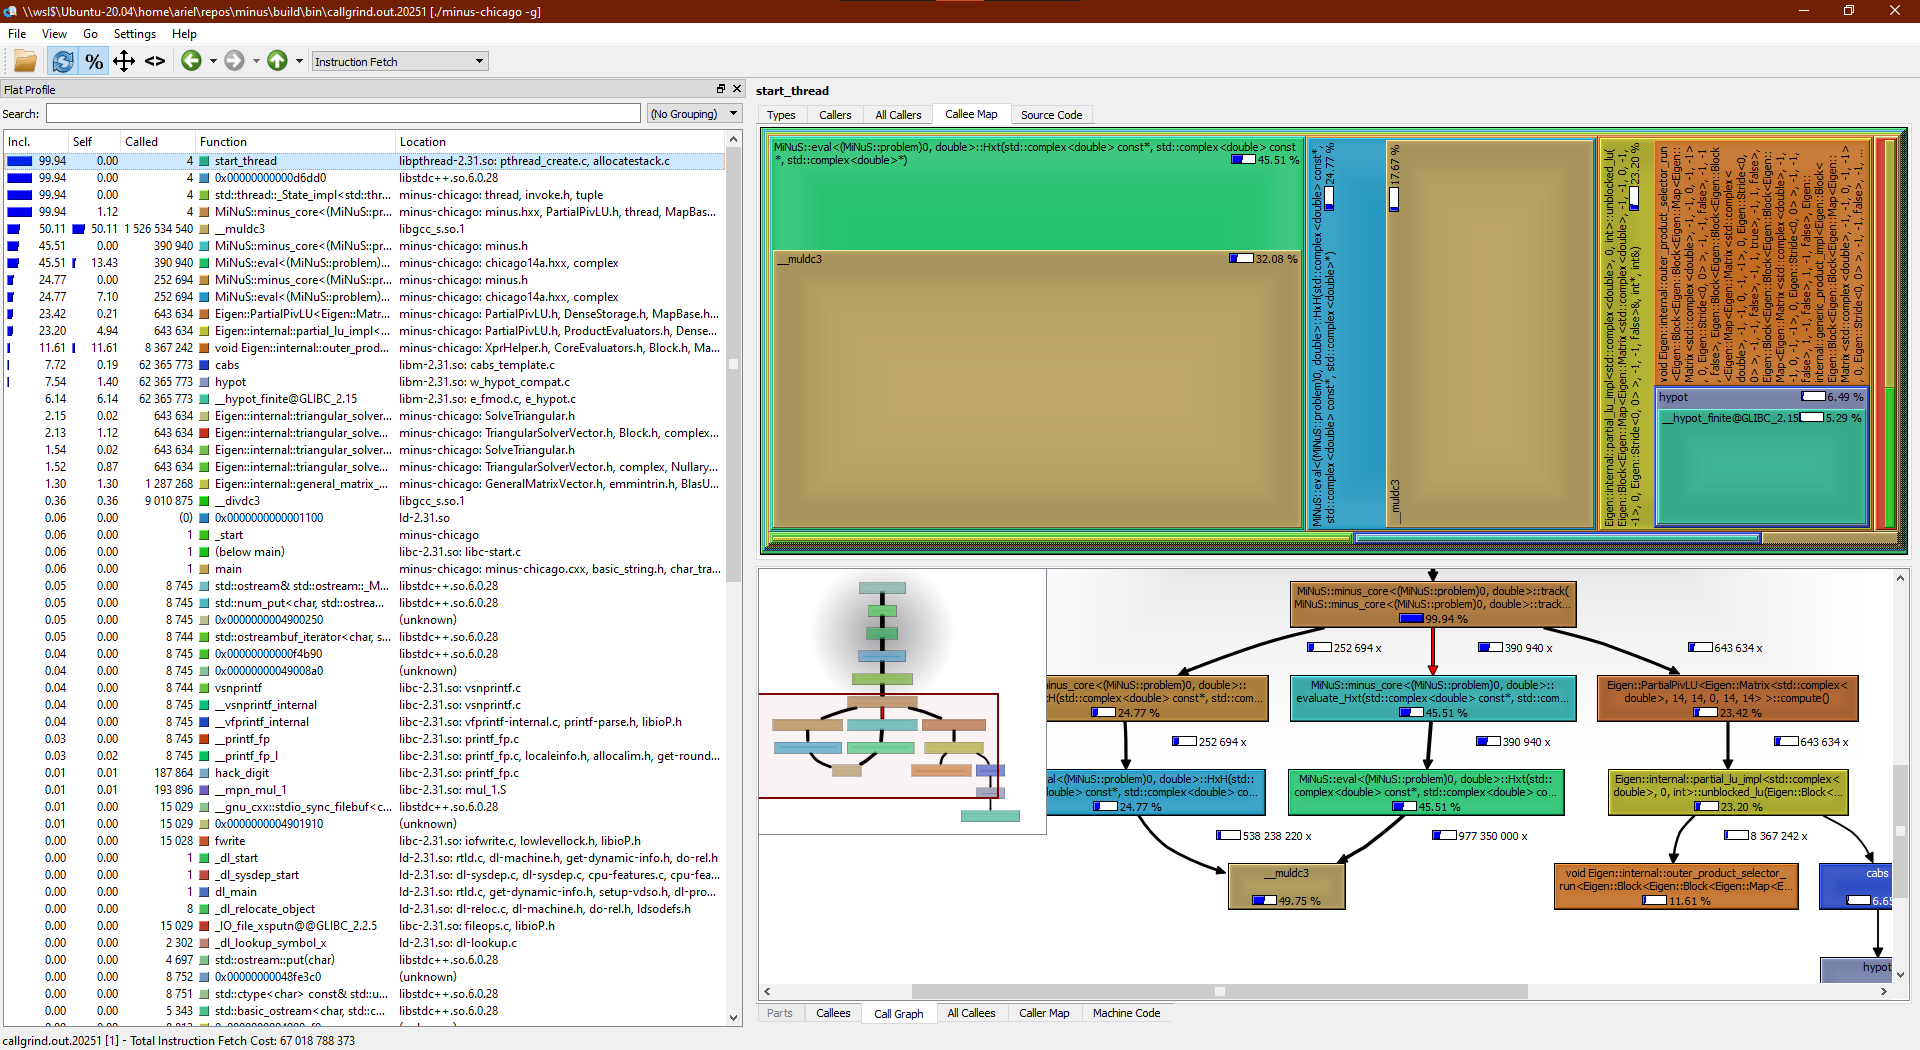
\includegraphics[width=\columnwidth]{figs/valgrind_qcachegrind_callgrind}
    \caption{Valgrind QCachegrind with Callgrind's output}
\end{figure}

\subsection{Further optimization strategies}

\subsubsection{Matrix Inversion}

We propose the predict and correct linear systems could be
more efficiently implemented via symbolic matrix inversion. 
This needs to be carefully implemented for the three point trifocal problem, as
14x14 size seems to lie on the limit where matrix inversion might or might not be feasible.

\subsubsection{Corrector steps using QR decomposition}

Solving linear systems using QR decomposition is more stable, according to our
experiments, than LU or standard Gaussian elimination. We have observed that
more corrector steps significantly speeds up the solver, but increases the
chance of failed solves due to path crossing when excessive correction is used.
It might make sense to use more stable or higher precision and stability in the
corrector step, while using less precision in the predictor step. One approach
would be to use LU decomposition with single precision for solving predictor
steps, while using QR decomposition with double precision for the corrector
steps. 
